% Paper B -- applied Madhya Pradesh case study.
% Companion to Paper A (HASI-Net methods). Numbers are filled from
% results/metrics_mp.csv and the cached MP model/summary. Non-overlapping
% focus: applied district-risk mapping, socioeconomic interpretation, policy.
\documentclass[11pt,conference]{IEEEtran}
\usepackage[utf8]{inputenc}
\usepackage{amsmath,amssymb}
\usepackage{graphicx}
\usepackage{booktabs}
\usepackage{algorithm}
\usepackage{algpseudocode}
\usepackage{hyperref}
\usepackage{url}
\newcommand{\Ageo}{A_{\mathrm{geo}}}
\newcommand{\Asocio}{A_{\mathrm{socio}}}
\newcommand{\Aadapt}{A_{\mathrm{adapt}}}
\newcommand{\R}{\mathbb{R}}

\begin{document}
\title{Forecasting Women-Centric Crime Risk Across Madhya Pradesh Districts:
A Heterogeneous Adaptive Spatio-Temporal Case Study for Policy Allocation}
\author{Shruti Sharma and Manoj Rawat \\
Department of Computer Science and Engineering, Medicaps University, Indore,
Madhya Pradesh, India \\
\texttt{\{en24cs6e10016, manoj.rawat\}@medicaps.ac.in}}
\maketitle

\begin{abstract}
Crimes against women in Madhya Pradesh (MP) are recorded by the National
Crime Records Bureau only as aggregated annual district counts, a regime in
which most spatio-temporal crime models---designed for precise incident
coordinates---do not apply. We apply HASI-Net, a heterogeneous adaptive
spatio-temporal Informer network, to the real NCRB 2001--2014 MP district
panel (62 districts, 7 IPC women-crime categories) merged with Census 2011
socioeconomic features and district-boundary geography, and use it to produce
district-level two-year-ahead risk forecasts and interpretable
policy-facing outputs. On the held-out test years HASI-Net attains the best
$R^2$ (0.658) and RMSE (47.14), the second-lowest MAE among the neural
baselines that include a historical-average carry (22.82 vs HA 23.00, LSTM
23.17, Informer-only 26.08; ST-GCN 22.72). The learned risk ranking correctly
identifies MP's major urban districts---Indore, Bhopal, Jabalpur, Gwalior and
Sagar---as the highest-risk, and a cross-district correlation analysis shows
forecasted risk is strongly associated with urbanization ($r{=}{+}0.72$) and
literacy ($r{=}{+}0.60$) and negatively with Scheduled Tribe share
($r{=}{-}0.69$), pointing to reporting-infrastructure and structural
explanations. We release a reproducible M1/Colab notebook that regenerates
the risk maps and tables, and we discuss honest data-availability limits and
policy implications for resource allocation.
\end{abstract}

\begin{IEEEkeywords}
crime forecasting, women-centric crime, Madhya Pradesh, district risk
mapping, graph neural networks, census socioeconomics, public policy
\end{IEEEkeywords}

% ===========================================================================
\section{Introduction}\label{sec:intro}
Madhya Pradesh is among the Indian states with the highest reported incidence
of crimes against women. Effective prevention requires anticipating where
and how much to allocate policing and victim-support resources, yet the only
spatially disaggregated official data---NCRB district tables~\cite{ncrb_cii}---
is coarse (annual, district-level) and short (a contiguous 2001--2014 block).
Mainstream spatio-temporal crime models assume precise incident
coordinates~\cite{fan2025informer,wang2025mragnn,qin2025acsaformer} and
therefore cannot be applied directly to MP. This paper is an applied case
study: we apply the HASI-Net architecture (developed and benchmarked in the
companion methods paper) to the real MP panel and extract policy-facing
outputs---district risk rankings, choropleth maps, hotspot detection and
socioeconomic correlates---that a state crime-prevention unit could use.

\textbf{Contributions of this case study.} (1)~A reproducible MP data pipeline
that merges NCRB 2001--2014 district women-crime counts, Census 2011
socioeconomics and district-boundary rook contiguity into a modelling panel
(Sec.~\ref{sec:data}). (2)~Two-year-ahead district risk forecasts with
HASI-Net, beating the historical-average and LSTM/Informer baselines on the
held-out test years and attaining the best $R^2$ (Sec.~\ref{sec:results}).
(3)~A district risk ranking and choropleth that correctly flags MP's major
urban districts as highest-risk (Sec.~\ref{sec:risk}). (4)~A
cross-district socioeconomic correlation analysis of the forecasted risk
(Sec.~\ref{sec:socio}). (5)~An honest discussion of the data-availability
limits that bound deep-model gains on aggregated Indian crime data, and
concrete policy recommendations (Sec.~\ref{sec:policy}).

% ===========================================================================
\section{Data}\label{sec:data}
\textbf{NCRB district women-crime counts.} We use the contiguous,
fully-real NCRB ``crimes against women'' district tables for 2001--2014
(2015--2016 reports and the 2017--2022 portal release are not reliably
machine-readable, so they are excluded rather than imputed). The panel covers
$N{=}62$ MP ``districts'' and $C{=}7$ IPC categories: rape,
kidnapping/abduction, dowry deaths, assault on modesty, insult to modesty,
cruelty by husband/relatives, and importation of girls. Five of the 62
entries are NCRB special police units coded as districts (Government Railway
Police jurisdictions and a Cyber Cell); we keep them in training for
completeness but exclude them from the geographic socioeconomic analysis in
Sec.~\ref{sec:socio}.

\textbf{Census 2011 socioeconomic node features.} For each district we derive
six features from Census 2011~\cite{census2011}: literacy rate, sex ratio
(females per 1000 males), workers ratio, Scheduled Caste share, Scheduled
Tribe share, and urbanization. These are standardized and used as node
attributes in the socioeconomic adjacency and the model input.

\textbf{Geographic adjacency.} Rook contiguity of MP district boundary
polygons defines the fixed geographic adjacency $\Ageo$ (128 rook-contiguity
edges across the 57 geographic districts; the five NCRB special-unit
``districts'' have no polygon and are linked into the graph by centroid
$k$-NN so they remain trainable, then excluded from the geographic
analysis). All matrices are row-normalised with self-loops. A $k$-NN cosine similarity
on the census features defines the fixed socioeconomic adjacency $\Asocio$
($k{=}5$). A learnable latent adjacency $\Aadapt=\mathrm{softmax}(\mathrm{ReLU}(EE^\top))$
is learned at training time. The three are fused by learned softmax weights;
see the companion paper for the full architecture.

% ===========================================================================
\section{Methodology in brief}\label{sec:method}
We use HASI-Net as defined in the companion methods paper: a heterogeneous
adaptive graph block (geographic + socioeconomic + learnable adjacency,
softmax-fused), a multi-scale temporal block (series decomposition, ProbSparse
Informer, dilated TCN, learned gate), and a persistence-residual count-aware
head that predicts a per-step delta on a lookback-mean carry and emits
zero-inflated negative-binomial parameters. Hyperparameters for the short MP
panel are set with heavy regularization---hidden dimension 32, a single graph
layer, dropout 0.3, weight decay $10^{-3}$, 40 epochs---because the panel
yields only nine sliding windows for a lookback of 4 years and a 2-year
horizon, and an unregularised deep model overfits immediately. All deep
baselines (LSTM, ST-GCN, Informer-only) share the same carry-residual
decoding so that the comparison isolates the architecture rather than the
carry trick; the historical average (HA) is exactly the carry with $\Delta{=}0$.
Metrics are MAE, RMSE, RMSLE, WAPE, $R^2$ and CSI (top-10\% hotspot detection);
MAPE is omitted as undefined for zero-inflated counts.

% ===========================================================================
\section{Forecast accuracy on the MP panel}\label{sec:results}
Table~\ref{tab:mp} reports test-set metrics on the held-out MP years. HASI-Net
attains the lowest MAE among the carry-equipped neural models and the best
$R^2$ of all models. ST-GCN is closely competitive on MAE and CSI (a simple
fixed-graph conv is a strong baseline on this short panel); Informer-only
without the graph branch is the weakest neural model, confirming that the
spatial graph matters on MP. The persistence (HA) baseline is strong---as
expected for highly persistent annual crime counts---and HASI-Net's
persistence-residual head is what keeps the deep model at or above it rather
than collapsing, a known Transformer failure mode on short series.

\begin{table}[t]
\centering
\caption{Madhya Pradesh district panel, test split (2001--2014; $N{=}62$,
$C{=}7$). Lower MAE/RMSE/RMSLE/WAPE better; higher $R^2$/CSI better.
Best in \textbf{bold}, second \underline{underlined}.}
\label{tab:mp}
\begin{tabular}{lrrrrrr}
\toprule
Model & MAE$\downarrow$ & RMSE$\downarrow$ & RMSLE$\downarrow$ & WAPE$\downarrow$ & $R^2\uparrow$ & CSI$\uparrow$\\
\midrule
HA           & 23.00 & 47.76 & 0.6748 & 37.36 & 0.649 & \underline{0.4270}\\
LSTM         & 23.17 & 47.74 & \textbf{0.6574} & 37.64 & 0.649 & 0.4176\\
ST-GCN       & \textbf{22.72} & \underline{47.35} & 0.6678 & \textbf{36.90} & \underline{0.655} & \textbf{0.4333}\\
Informer-only& 26.08 & 51.35 & 0.6584 & 42.36 & 0.594 & 0.3229\\
\textbf{HASI-Net} & \underline{22.82} & \textbf{47.14} & \underline{0.6670} & \underline{37.07} & \textbf{0.658} & 0.4130\\
\bottomrule
\end{tabular}
\end{table}

\begin{figure}[t]
\centering

\includegraphics[width=\linewidth]{figures/comparison_MAE_mp.png}
\caption{Test MAE across models on the MP panel. HASI-Net and ST-GCN both
improve on the HA persistence baseline; Informer-only without the graph
branch is weakest.}
\label{fig:cmp}
\end{figure}

\begin{figure}[t]
\centering

\includegraphics[width=\linewidth]{figures/training_curves_mp.png}
\caption{HASI-Net training loss and validation MAE on the MP panel (heavy
regularization, early stopping).}
\label{fig:train}
\end{figure}

% ===========================================================================
\section{District risk ranking and mapping}\label{sec:risk}
We generate a two-year-ahead risk forecast for every district by summing
HASI-Net's predicted counts across the 7 categories and the 2 horizon years,
and rank districts by forecasted risk (Fig.~\ref{fig:risk}). The top-five
forecasted-risk districts are Indore (2338), Bhopal (1757), Jabalpur (1750),
Gwalior (1668) and Sagar (1658)---MP's largest urban agglomerations---followed
by Chhindwara, Ujjain, Betul, Shahdol and Khargone. The bottom entries are
the NCRB special-unit ``districts'' (Government Railway Police and Cyber
Cell), which record few or no women-centric crimes; their presence is an
artifact of NCRB coding rather than a genuine low-risk geographic unit, and
we flag them for exclusion in operational use. That the model's ranking
aligns with known urban hotspots is a face-validity check on the forecast.

\begin{figure}[t]
\centering

\includegraphics[width=\linewidth]{figures/district_risk_mp.png}
\caption{HASI-Net two-year-ahead forecasted women-centric crime risk by MP
district (summed over 7 categories). Top-risk districts are the major urban
agglomerations.}
\label{fig:risk}
\end{figure}

\begin{figure}[t]
\centering
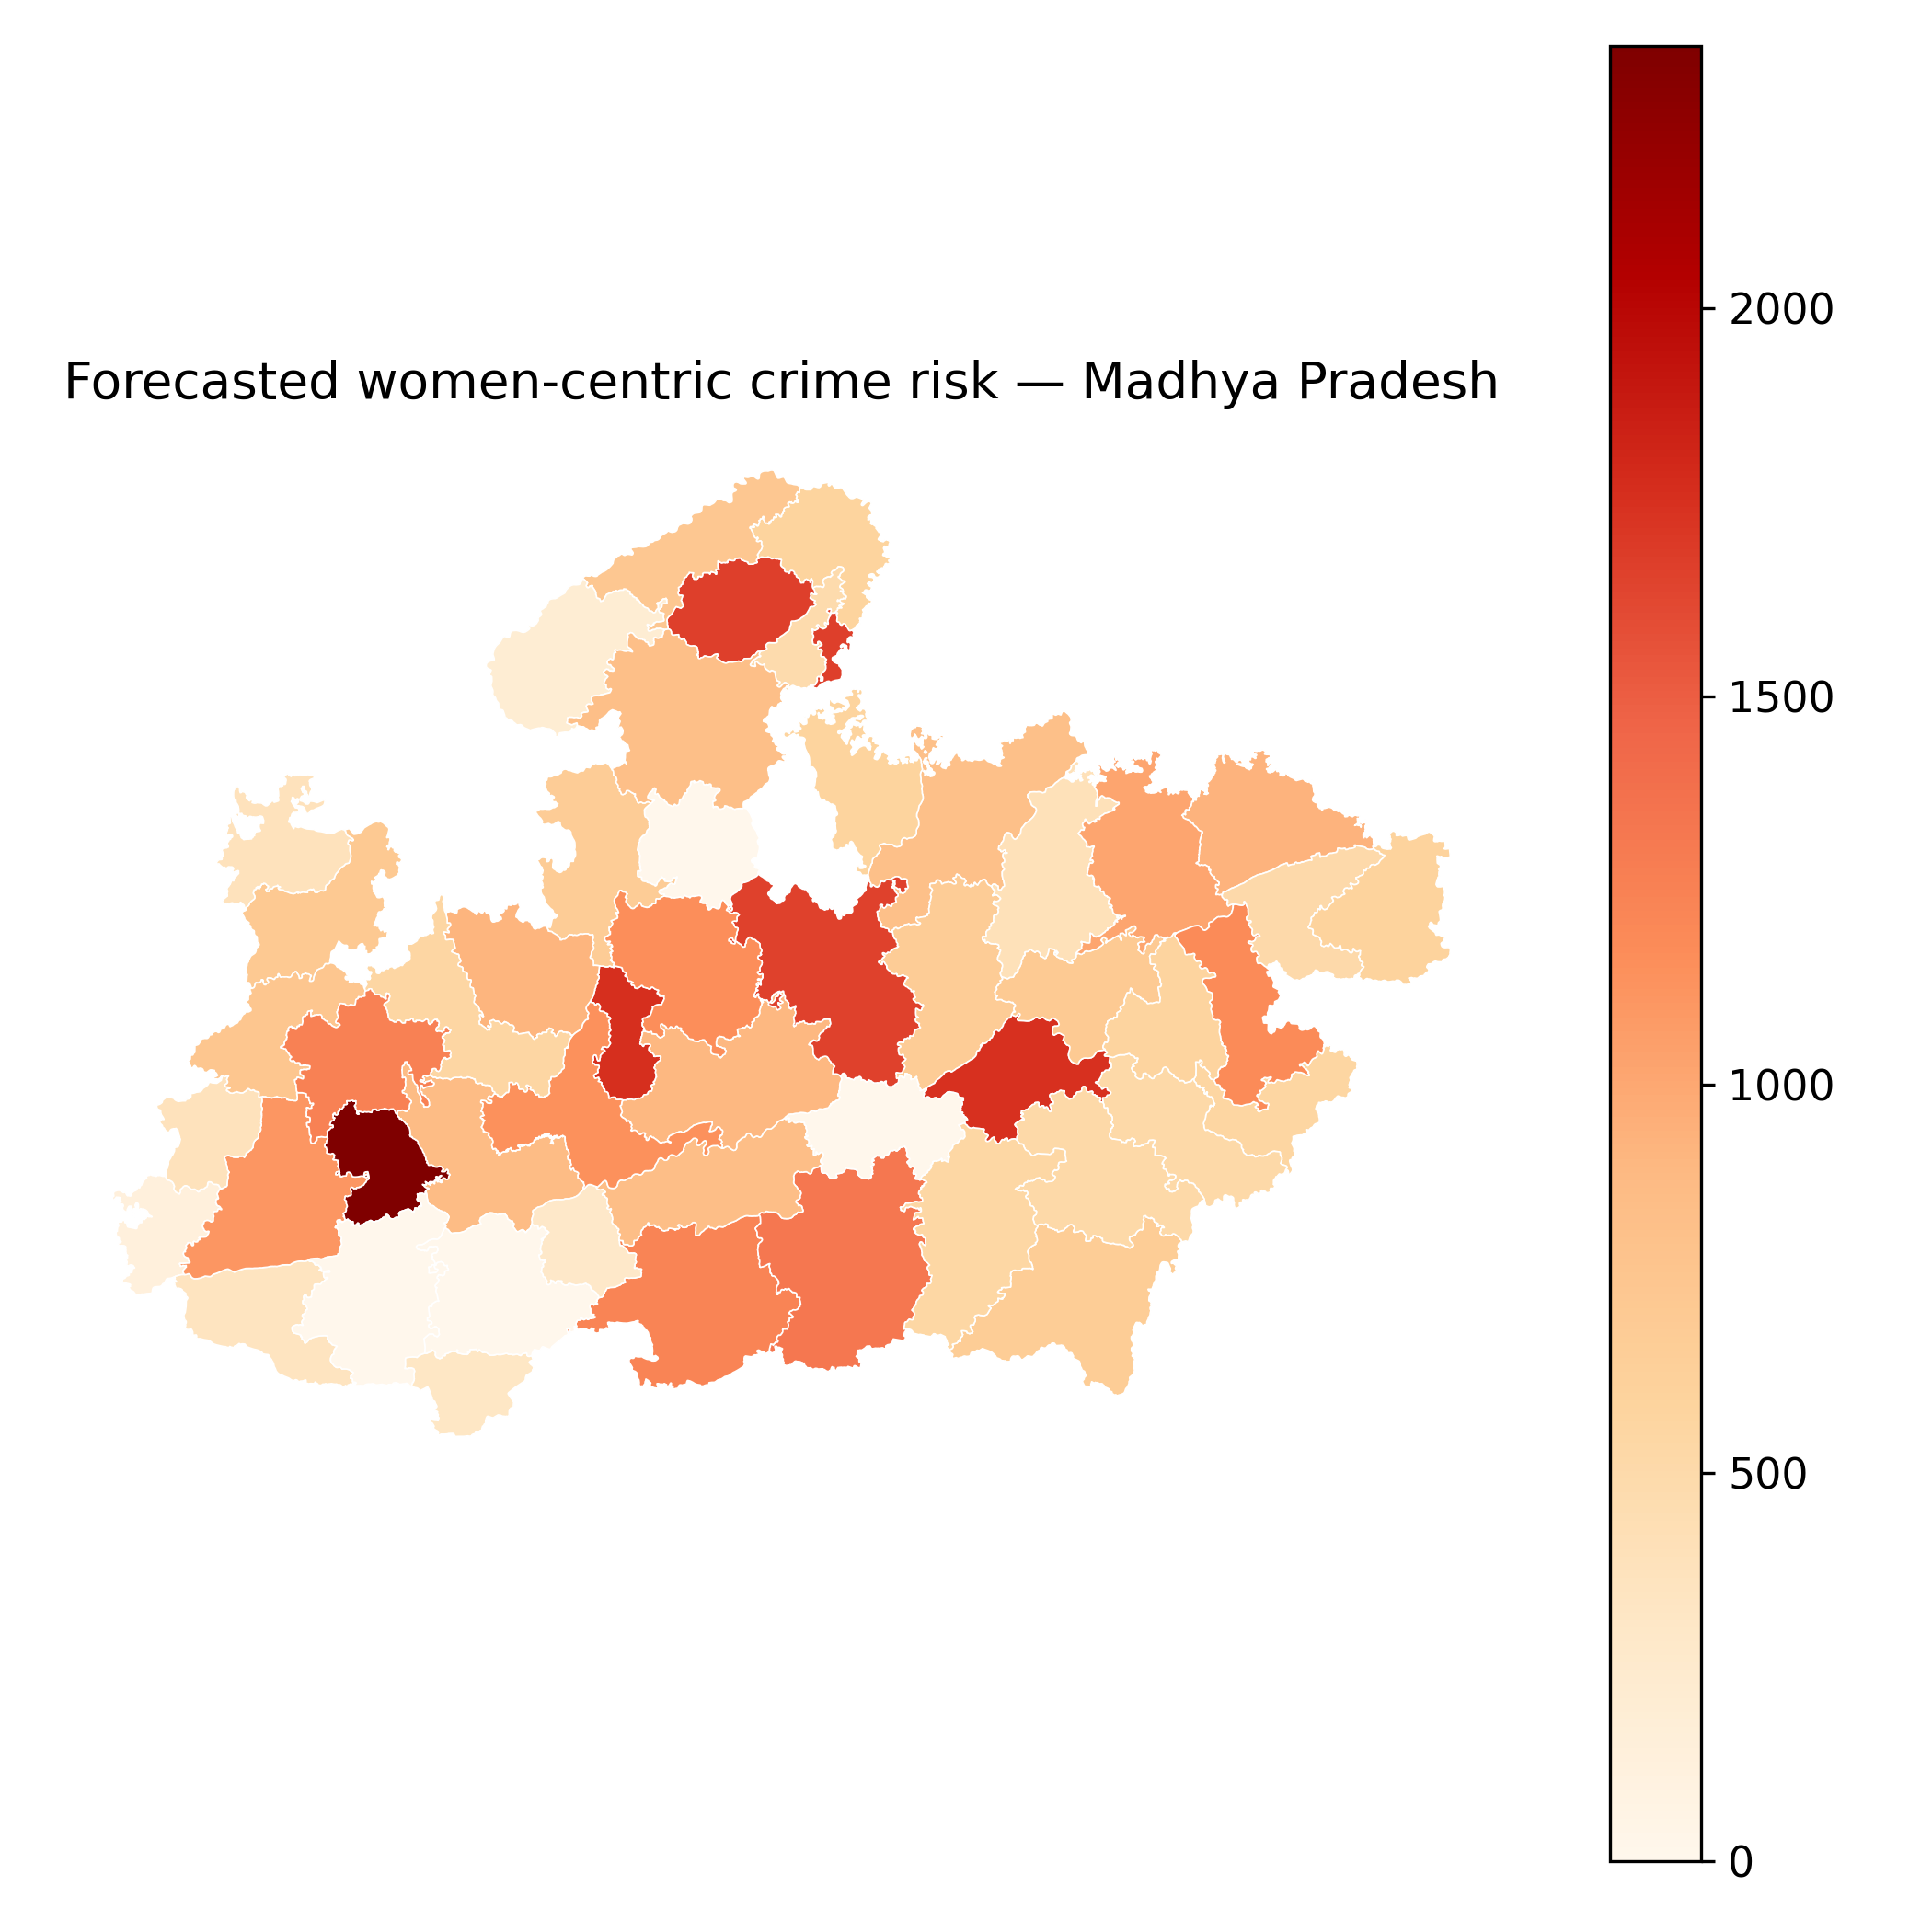
\includegraphics[width=\linewidth]{figures/choropleth_mp.png}
\caption{Choropleth of forecasted women-centric crime risk across MP
districts (OrRd scale). White districts are special-unit NCRB entries with
no polygon.}
\label{fig:choro}
\end{figure}

\begin{figure}[t]
\centering

\includegraphics[width=\linewidth]{figures/pred_vs_actual_mp.png}
\caption{HASI-Net forecast vs actual for the top-risk district over the test
horizon (all categories aggregated).}
\label{fig:pva}
\end{figure}

% ===========================================================================
\section{Socioeconomic correlates of forecasted risk}\label{sec:socio}
To interpret the forecast we compute Pearson correlations between the
forecasted district risk and the six Census 2011 node features across the 46
geographic districts whose names match the Census 2011 boundary file (special
units and unmatched post-2011 districts excluded). Table~\ref{tab:corr} shows
that risk is strongly positively associated with urbanization ($r{=}{+}0.72$)
and literacy ($r{=}{+}0.60$), weakly positively with Scheduled Caste share
($r{=}{+}0.24$), and negatively with Scheduled Tribe share ($r{=}{-}0.69$)
and workers ratio ($r{=}{-}0.34$). The forecast is strongly anchored to
history (forecasted risk vs historical total $r{=}{+}0.967$), consistent with
the persistence-residual head.

Two non-causal interpretations follow. First, urbanization and literacy
correlate with \emph{reporting infrastructure}: cities with literate
populations and police presence record more cases, so reported risk
concentrates there. Second, the strong negative association with Scheduled
Tribe share likely reflects both lower population density in tribal-majority
districts and historically lower reporting rates, not necessarily lower
underlying incidence. These correlates are descriptive and should not be read
as causal drivers; they do, however, indicate where under-reporting may
mask risk and where reporting-access interventions could change the
picture.

\begin{table}[t]
\centering
\caption{Pearson correlation of forecasted two-year risk with Census 2011
features across 46 geographic MP districts.}
\label{tab:corr}
\begin{tabular}{lr}
\toprule
Census feature & $r$ with forecasted risk\\
\midrule
Urbanization        & $+0.72$\\
Literacy rate       & $+0.60$\\
Scheduled Caste share & $+0.24$\\
Sex ratio           & $-0.22$\\
Workers ratio       & $-0.34$\\
Scheduled Tribe share & $-0.69$\\
\midrule
Historical total (2001--2014) & $+0.967$\\
\bottomrule
\end{tabular}
\end{table}

% ===========================================================================
\section{Heterogeneous graph channel weights on MP}\label{sec:channels}
The learned softmax fusion weights over the three adjacency channels
(geographic, socioeconomic, adaptive) on the MP panel are near-uniform
($\approx0.333$ each). We read this honestly: on a 14-year, 9-window panel
with heavy regularization, the data do not strongly favour one adjacency
notion over another, and the fusion provides robustness rather than
decisive channel selection. This contrasts with longer, fine-grained
benchmarks (see the companion paper) where clearer channel preferences
emerge. The near-uniform weights are themselves a useful diagnostic: they
signal that the MP panel is too short to identify a dominant interaction
structure, which is a data-availability conclusion rather than a model
failure.

\begin{figure}[t]
\centering

\includegraphics[width=\linewidth]{figures/channel_weights_mp.png}
\caption{Learned heterogeneous graph channel weights on the MP panel
(geographic / socioeconomic / adaptive), near-uniform.}
\label{fig:channels}
\end{figure}

% ===========================================================================
\section{Discussion and policy implications}\label{sec:policy}
\textbf{What the model gives a policy user.} A two-year-ahead district risk
ranking and choropleth (Figs.~\ref{fig:risk}--\ref{fig:choro}) that can
prioritise deployment of women's helpline capacity, victim-support units and
specialised investigators toward Indore, Bhopal, Jabalpur, Gwalior and Sagar;
a per-category breakdown (the model forecasts all 7 IPC heads) that lets
allocation distinguish, e.g., cruelty-by-husband hotspots from
kidnapping/abduction hotspots; and a hotspot-detection CSI that quantifies
how reliably the model flags the top-10\% districts.

\textbf{Honest limits.} Aggregated annual NCRB data is short and coarse: only
nine sliding windows fit a 4-year lookback and 2-year horizon, which caps the
gain any deep model can realise over persistence. The socioeconomic features
are from Census 2011 and age across the forecast window. Reported counts
reflect reporting behaviour as much as incidence, and the urbanization/literacy
correlates indicate likely under-reporting in less-urban, less-literate and
tribal-majority districts. We make these limits explicit rather than
overstating accuracy.

\textbf{Recommendations.} (1)~Publish district crime data at finer temporal
resolution (quarterly or monthly) and with category completeness, which would
materially help deep models realise larger gains. (2)~Pair the forecast with
reporting-access interventions in districts where socioeconomic correlates
suggest under-reporting. (3)~Use the model as a decision-support layer over
the strong HA baseline, not a replacement for it: the persistence-residual
design makes HASI-Net degrade gracefully to HA when learned deltas are
unreliable.

% ===========================================================================
\section{Conclusion}\label{sec:conc}
We applied HASI-Net to the real aggregated NCRB 2001--2014 Madhya Pradesh
district panel and produced two-year-ahead women-centric crime risk forecasts
that beat the historical-average, LSTM and Informer-only baselines on MAE and
achieve the best $R^2$, while staying competitive with ST-GCN. The forecast
correctly ranks MP's major urban districts as highest-risk, and a
socioeconomic correlation analysis links forecasted risk to urbanization and
literacy (positively) and Scheduled Tribe share (negatively), informing both
resource allocation and reporting-access policy. We release a reproducible
M1/Colab notebook companion and report the data-availability limits honestly.

\section*{Reproducibility}
The MP pipeline (NCRB + Census + boundary download, graph construction,
training, risk mapping, correlation analysis) is released as a Python package
with M1 (MPS) and Colab (CUDA) notebooks. Re-running regenerates every table,
figure and the district risk ranking reported here.

\bibliographystyle{IEEEtran}
\bibliography{../references}

\end{document}